\documentclass{beamer}
\usepackage{graphicx}
\usepackage{amsmath}
\usepackage{amsfonts}
\usepackage{amssymb}
\usepackage{pdfpages}
\usepackage[all]{xy}
\usetheme{AISEC}
\setbeamercovered{transparent}

% Load Fraunhofer font
\IfFileExists{fhgfon.tsty}
{
    \usepackage{fhgfont}
}
{
    % Font Settings: rev. Times, rev. Helvetica and DejaVuSansMono
    \usepackage[notext]{stix}
    \usepackage{tgtermes}
    \usepackage[scale=0.92]{tgheros}
    \usepackage[scaled=0.80]{DejaVuSansMono}
}

% Better typography
\usepackage[
    activate={true,nocompatibility},
    final,
    tracking=true,
    kerning=true,
    spacing=true,
    babel=true,
]{microtype}

% Codelistings
% \usepackage[]{minted}
% \usemintedstyle{bw}

% Configure linenumbers of code blocks
% \renewcommand{\theFancyVerbLine}{
%     \sffamily
%     \textcolor{black}{\scriptsize\arabic{FancyVerbLine}}
% }
%
% Example for a minted python environment:
% \newminted{python}{
%     fontsize=\normalsize,
%     numbersep=10pt,
%     xleftmargin=1pt,
%     xrightmargin=1pt
% }

% Load and set up input encoding and babel
\usepackage[utf8]{inputenc}
\usepackage[english]{babel}

% Load and set up other packages
%\graphicspath{{./figures/}} % Set the search path for graphics


% Configure Fraunhofer beamer theme

% Disable the infoline in the footer [default: enabled]
% \infolinefalse

% Enable automatic numbering of frame titles and subtitles;
% used in conjunction with sectioning [default: disabled]
% \numberingtrue

% Disable the use of squares in itemize environments [default: enabled]
% \usesquaresfalse

% Disable the extended title page headline [default: enabled]
% \extendedtitlefalse

% Display  red CONFIDENTIAL string in the infoline [default: disabled]
% \confidentialtrue


% Set title page infromation
\title[Short Title]{Post-quantum secure PUF authentication using LPN}
\subtitle[Short Subtitle]{ }
\author[Short Author]{Han Zhao}
\date{\today}


% Set contact page information
\name{\insertauthor}
\department{Group Product Protection\newline Department Security and Trusted OS}
\institute{Fraunhofer-Institute for\newline Applied and Integrated Security (AISEC)}
\address{Parkring 4\newline 85748 Garching (near Munich)\newline Germany}
\web{http://www.aisec.fraunhofer.de}
\phone{+49 16 25231418}
\fax{+49 89 3229986-222}
\email{ga84fif@mytum.de}


\begin{document}

\begin{titleframe}
    \titlepage
    \vskip2.7cm
    \begin{center}
        
\includegraphics[scale=.7]{aisec_logo.pdf}
    \end{center}
\end{titleframe}

\begin{outlineframe}
%    \frametitle{Outline}
    \tableofcontents
\end{outlineframe}

% Content
\section{Introduction}

\begin{outlineframe}
	\tableofcontents[currentsection]
\end{outlineframe}
\subsection{Concept}
\begin{frame}
	\alert{LPN}:  Learning Parity with Noise \\
	\vspace{0.2cm}
	\begin{description}
		\item[1.] Randomly select a secret \alert{s} in GF(2)
		\item[2.] Randomly select \alert{A} from GF(2)
		\item[3.] Select a noise \alert{e} $\longrightarrow$ $Ber_{\epsilon}$
%			$\xymatrix@1{ \ar@{->|}[r] & }$ $Ber_\epsilon}$
		\item[4.] Output \alert{b}= $<$ A*s+e $>$ as a sample\\
				$b_{i} = A_{i}$*$s+e_{i}$ ~~~~mod~~2~~~~with i={0,1,...,m}\\
	\end{description}
	\vspace{0.2cm}
			\vspace{0.5cm}		
	The goal: \\
	\vspace{0.2cm}
	\centering
	Find s given only the values of b and A.\\ 
\end{frame}





\subsection{Motivation}
\begin{frame}
	\begin{itemize}
		\item Fundamental in theory%strong PUF VS weak PUF
		\begin{itemize}
			\item A close connection to the problem of decoding binary random linear codes.
			\item Believed to be hard: no polynomial time algorithm is known.
		\end{itemize}	
	\end{itemize}
%
%	\vspace{0.2cm}
%	\begin{itemize}
%		\item Many cryptographic applications in practice %% LPN -- NP Problem
%		\begin{itemize}
%			\item User authentication, encryption, etc.
%			\item Post-quantum cryptography.%Traditional Encryption VS One-time-pad
%		\end{itemize}
%	\end{itemize}
%	\begin{itemize}
%		\item Traditional Encryption VS One-time-pad
%	\end{itemize}
%	\vspace{0.2cm}
\end{frame}


\begin{frame}
	\frametitle{Motivation}
	\framesubtitle{LPN -- Problem}
	1. BKW Algorithm$^{1}$\\
	labeled examples: $ 2^{\Omega\left(\frac{n}{logn}}\right) $ \\
	time consuption: $ 2^{\Omega\left({\frac{n}{logn}}}\right) $\\
	\vspace{0.3cm}
	2. Algorithm of Lyubashevsky$^{2}$ \\
	labeled examples: $n^{1+\epsilon}$ \\
	time consuption: $ 2^{\Omega\left({\frac{n}{log logn}}} \right)$ \\
	\vspace{0.3cm}
	3. LF1 Algorithm$^{3}$ \\
	labeled examples: polynomial number of trials \\
	time consuption: exponential time\\
	\vspace{0.5cm}
\end{frame}


%\subsection{Motivation}
\begin{frame}
	\begin{itemize}
		\item Fundamental in theory%strong PUF VS weak PUF
		\begin{itemize}
			\item A close connection to the problem of decoding binary random linear codes.
			\item Believed to be hard: no polynomial time algorithm is known.
		\end{itemize}	
	\end{itemize}
	
	\vspace{0.2cm}
	\begin{itemize}
		\item Many cryptographic applications in practice %% LPN -- NP Problem
		\begin{itemize}
			\item User authentication, encryption, etc.
			\item Post-quantum cryptography.%Traditional Encryption VS One-time-pad
		\end{itemize}
	\end{itemize}
	%	\begin{itemize}
	%		\item Traditional Encryption VS One-time-pad
	%	\end{itemize}
	%	\vspace{0.2cm}
\end{frame}


%\subsection{Notation}
%\begin{frame}
%	\alert{TRNG}: True Random Number Generator\\
%	\vspace{0.2cm}
%	\alert{A}: publicly known matrix (Generator Matrix)\\
%	\vspace{0.2cm}
%	\alert{e}: the initial reference response of PUF\\
%	\vspace{0.2cm}
%	\alert{e{'}}: the PUF response of the identical challenge in later time\\
%\end{frame}



\section{The construction of the authentication system}


\begin{outlineframe}
	\tableofcontents[currentsection]
\end{outlineframe}
\begin{frame}
%	\framesubtitle{The first stage}
	Enrollment phase:
	\begin{itemize}
		\item Collecting response and chanllenge pairs (RCPs)
		\begin{itemize}
			\item Encoding module
		\end{itemize}
	\end{itemize}
	Authentication phase:
	\begin{itemize}
		\item Matching the extracted RCPs with the reference RCPs 
		\begin{itemize}
			\item Decoding module
		\end{itemize}
	\end{itemize}
\end{frame}

\subsection{Enrollment phase}
\begin{frame}
    \frametitle{The construction of the authentication system}
    \framesubtitle{Enrollment phase}
%    \begin{alertenv}
%    	Reference challenge-response pairs are collected:
%    \end{alertenv}
    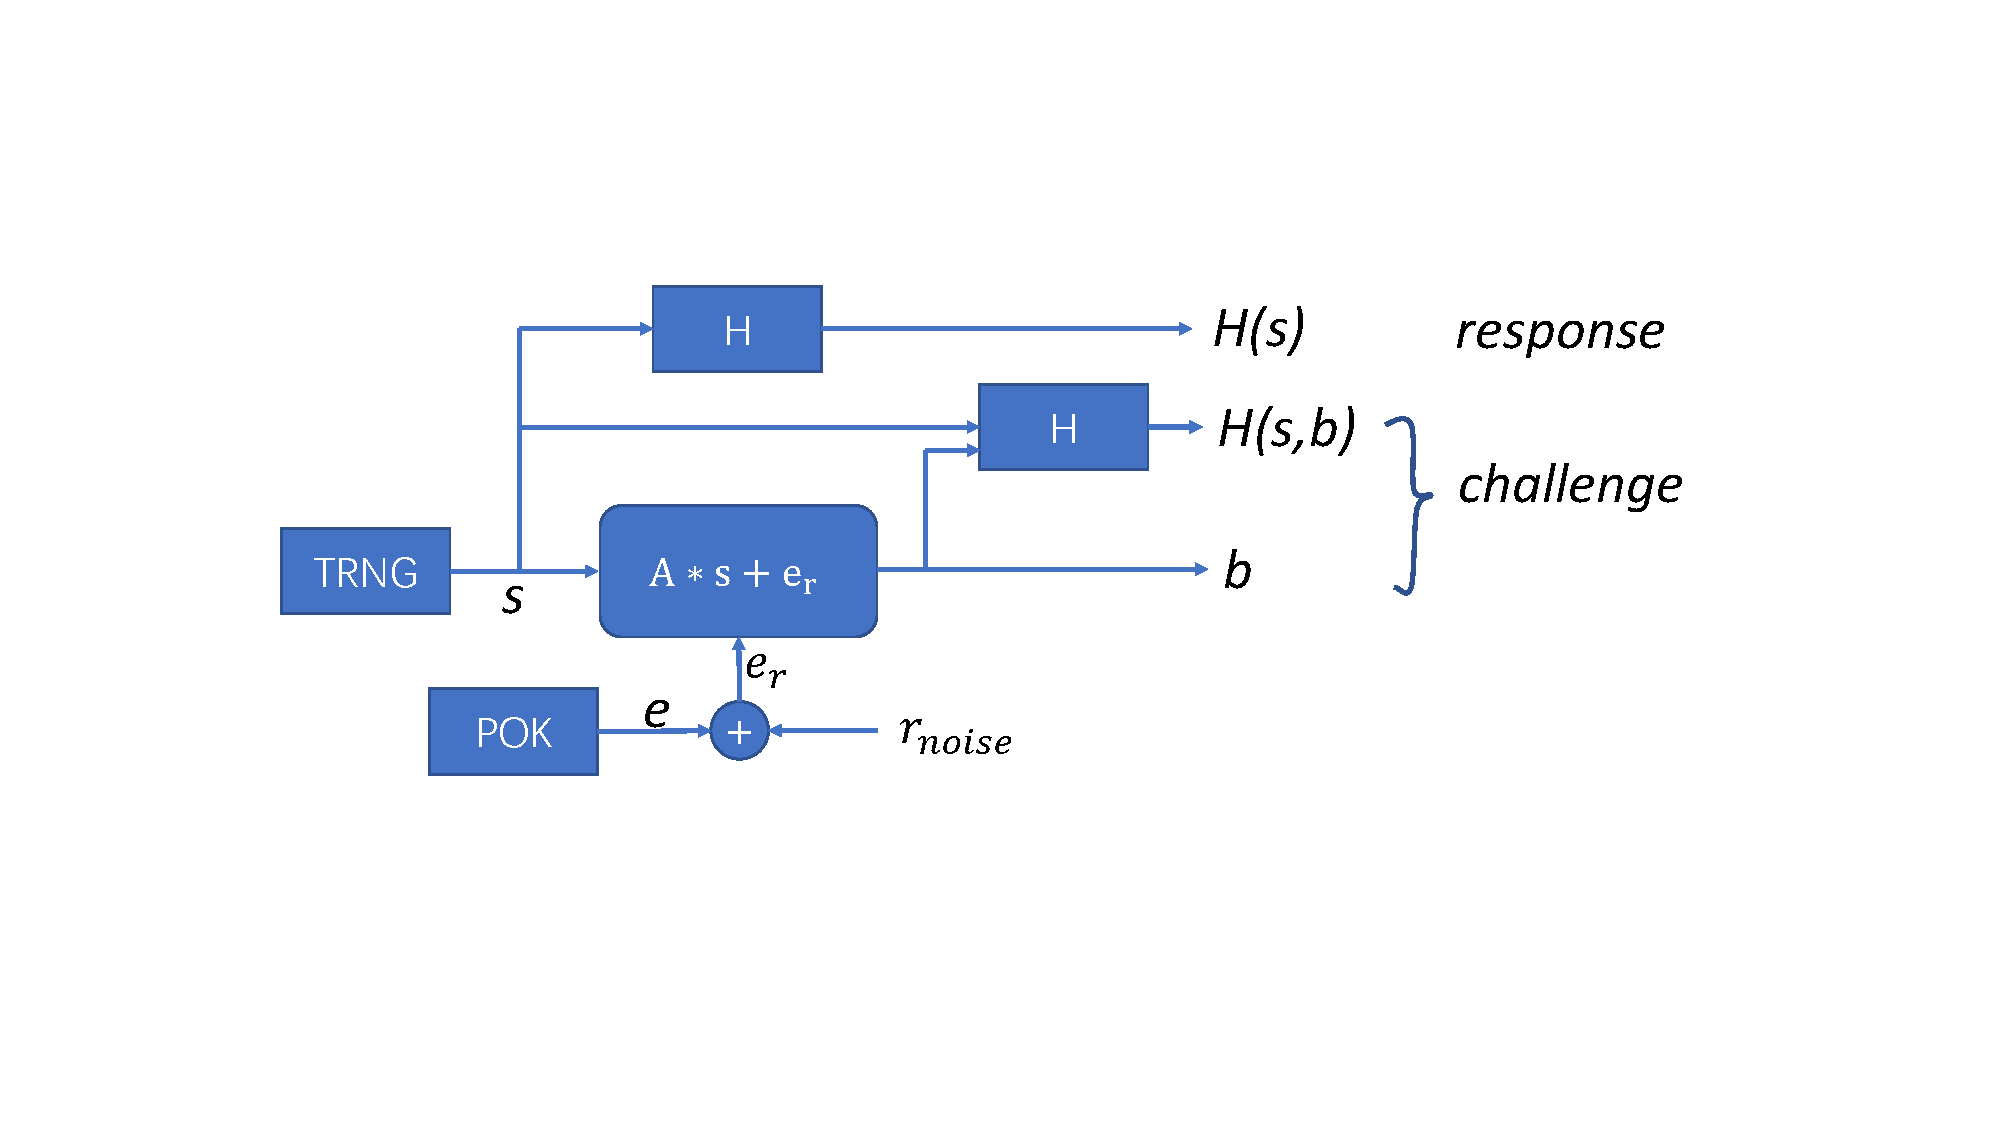
\includegraphics[width=5in,height=3in]{Enrollment-phase.pdf}
\end{frame}


\subsection{Authentication phase}
\begin{frame}
	\frametitle{The construction of the authentication system}
	\framesubtitle{Authentication phase}
	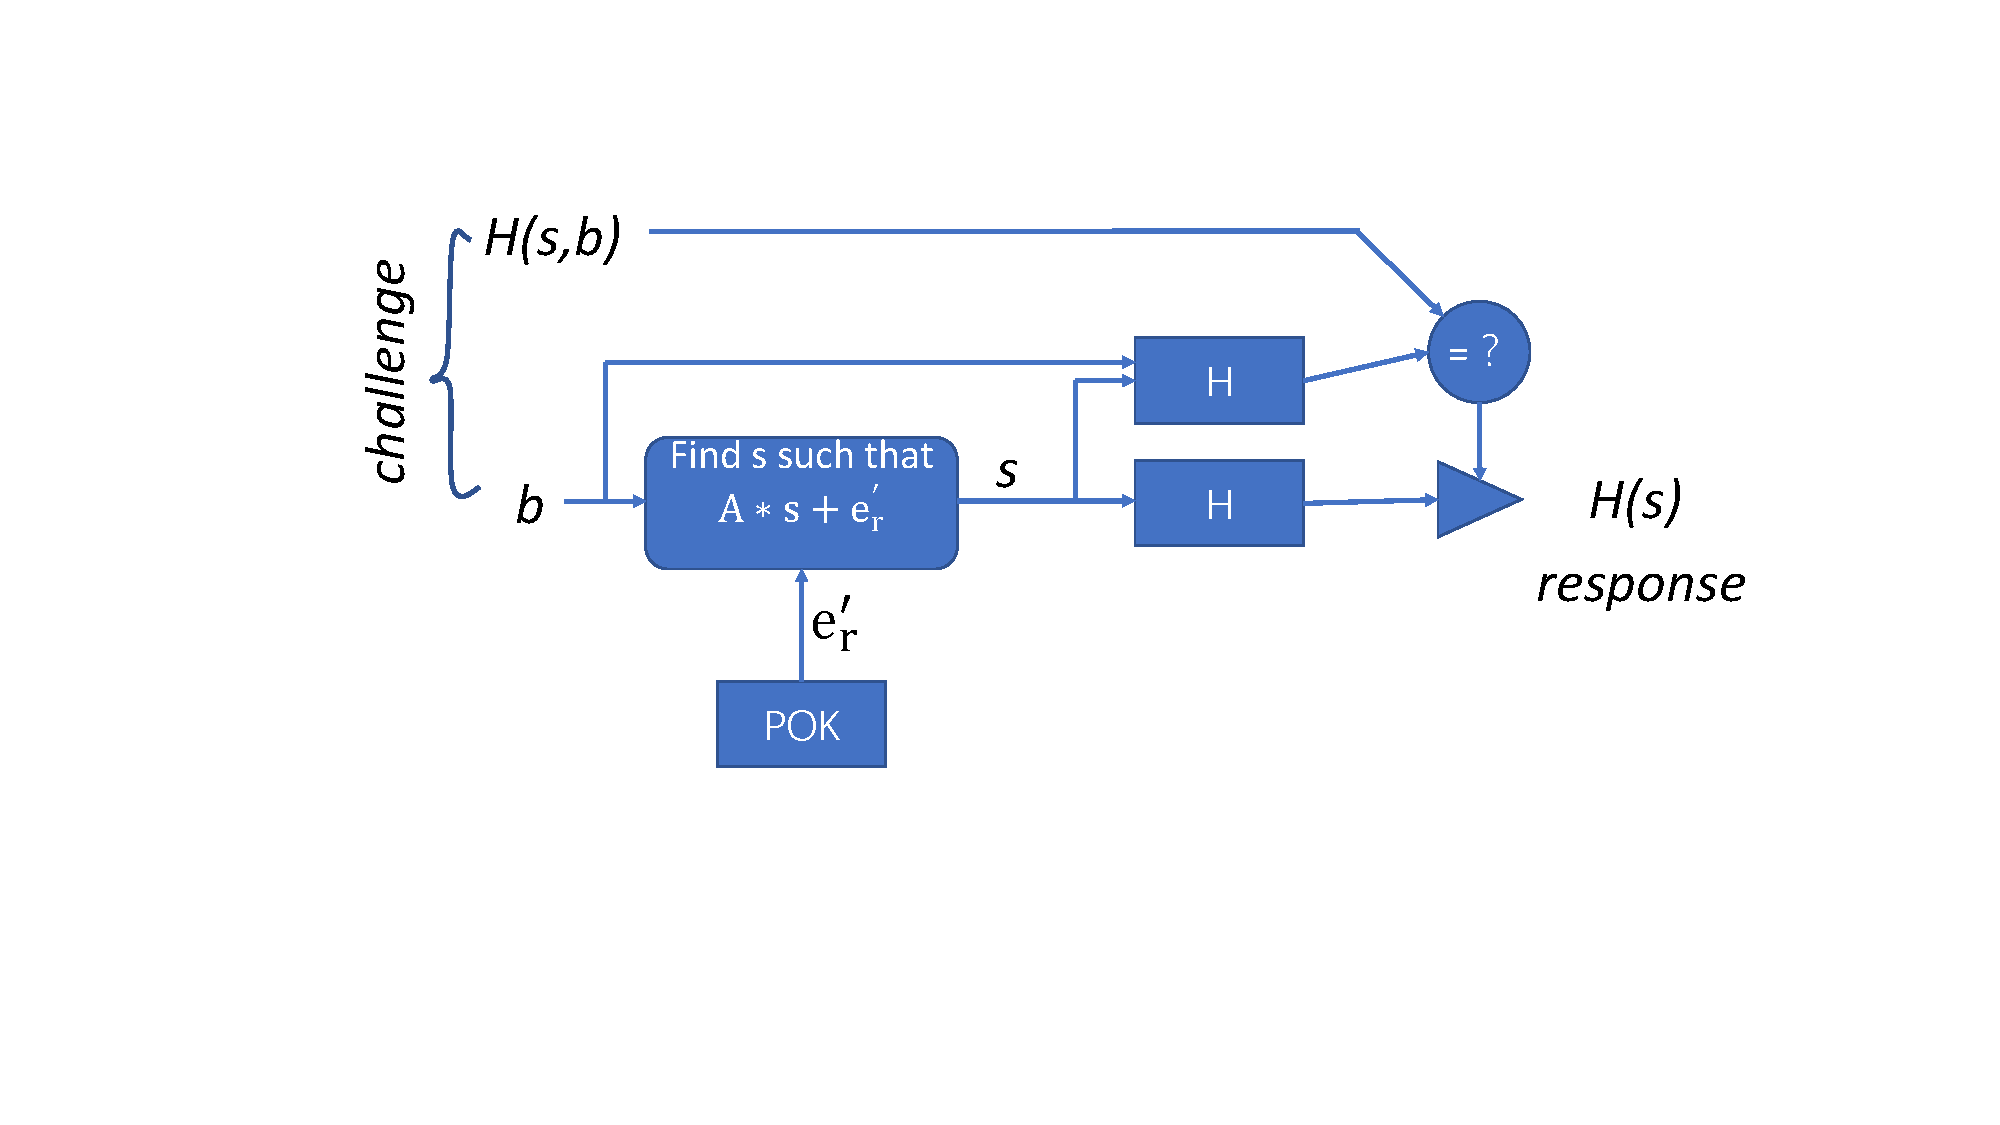
\includegraphics[width=5in,height=3in]{Authentication-phase.pdf}
\end{frame}


\begin{frame}
	\frametitle{The construction of the authentication system}
	\framesubtitle{Authentication phase}
	{\Large	Extracting s from the decoding module:}\\
	\vspace{0.5cm}
	\begin{itemize}
		\item Gaussian elimination algorithm 
	\end{itemize}
	\begin{itemize}
	\item Error correction algorithm
	\end{itemize}
	
\end{frame}


\begin{frame}
	\frametitle{Authentication phase}
	\framesubtitle{Error correction codes}
	{\Large Possible Candidates:}\\
	\vspace{0.5cm}
	Hamming Code\\
	\vspace{0.3cm}
	Repetition Code\\
	\vspace{0.3cm}
	BCH Code\\
	\vspace{0.3cm}
	Reed-Muller Code\\
	\vspace{0.3cm}
	LDPC Code\\	
\end{frame}

\begin{frame}
	\frametitle{Error correction code}
	\framesubtitle{Reed Muller Code}
	{\Large Characteristics:}\\
	\begin{itemize}
		\item the simple construction
	\end{itemize}
	\begin{itemize}
		\item no parity check matrix
	\end{itemize}
	\begin{itemize}
	\item good error correction property
	\end{itemize}
\end{frame}



\begin{frame}
	\frametitle{Encoding Algorithm}
	\framesubtitle{The Plotkin-Construction^{4}}
	Characterization of RM(r,m) codes with the parameters r and m:\\
	\vspace{0.2cm}
	$n=2^{m}$	\\
	\vspace{0.2cm}
	$k=\sum_{i=1}^r $$\left(\begin{aligned} m\\i \end{aligned} \right) $   \\
	\vspace{0.2cm}
	$ d = {2^{m \textnormal{-} r}} $ \\
Plotkin construction with two subcodes for RM(r,m):\\
	\vspace{0.2cm}
%	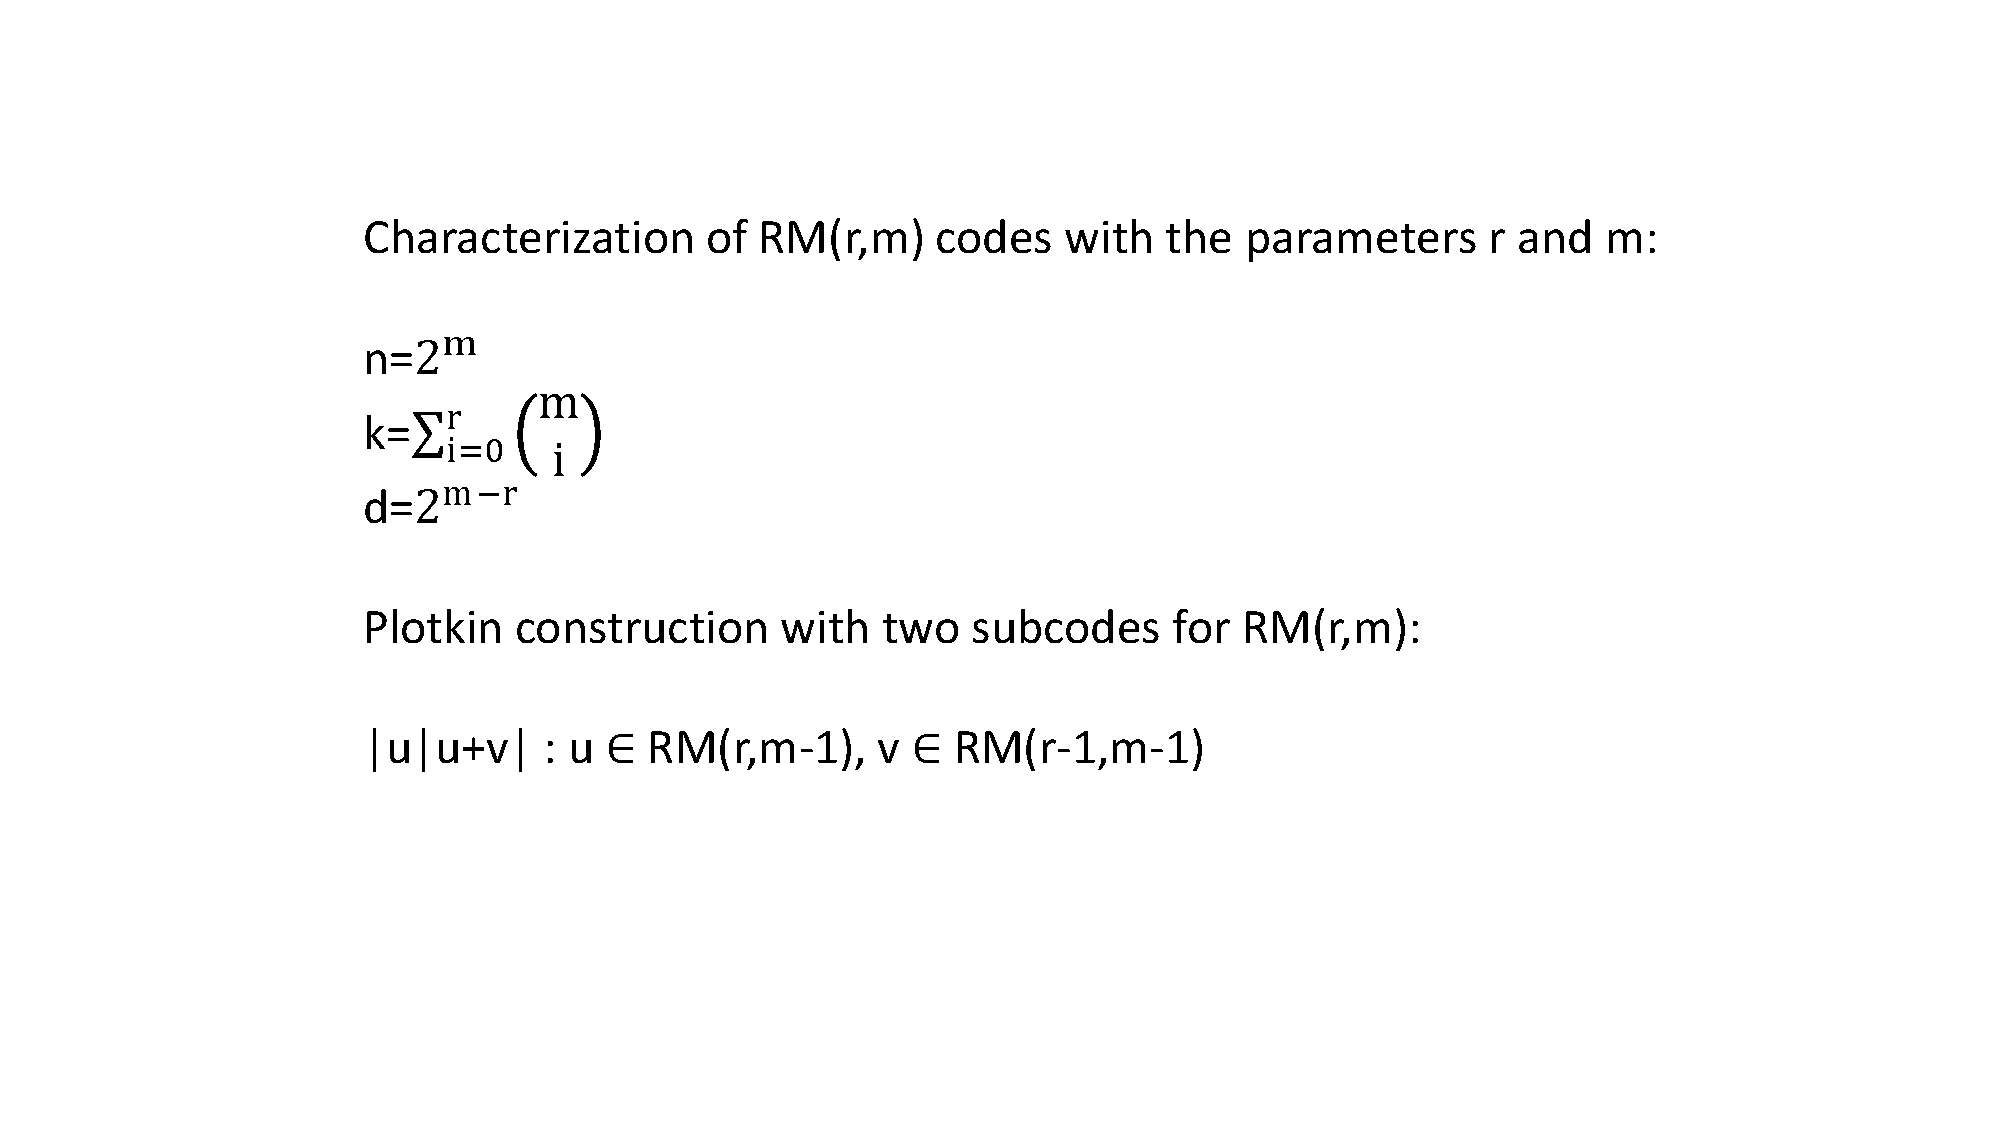
\includegraphics[width=5in,height=3.5in]{Plotkin-Construction.pdf}
	$\left| u\right|$ $\left u + v \right| $	 $:$	u  $\epsilon$ RM(r,m{-}1), v $\epsilon$ RM(r{-}1,m{-}1)
\end{frame}

\begin{frame}
	\frametitle{Reed Muller Code}
	\framesubtitle{RM(1,7)}
%	\framesubsubtitle{RM(4,7):}
	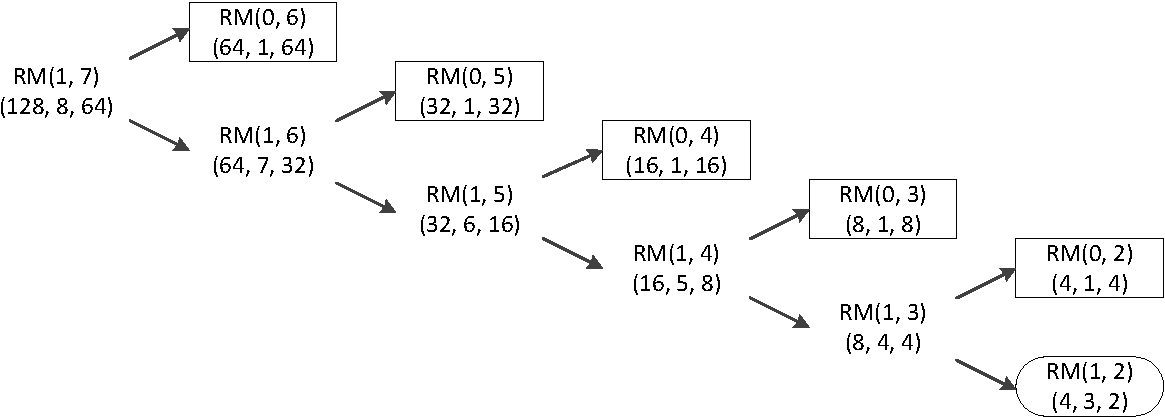
\includegraphics[width=4.2in,height=2.8in]{Baum_RM17.pdf}
\end{frame}


\begin{frame}
	\frametitle{Decoding Algorithm}
	\framesubtitle{The Recursive Decoding Algorithm^{4}}
	\begin{description}
	\item [1 )]SDML-Decoding for Repetition Code or Parity-Check Code
	\end{description}
	\begin{description}
	\item [2a)]Decoding for the first outer codeword RM(r-1,m-1)
	\end{description}
	\begin{description}
	\item [2b)]Decoding for the second outer codeword RM(r,m-1)
	\end{description}
	\begin{description}
	\item [3)]Reconstructing the codeword RM(r,m) with the two subcodes
	\end{description}
\vspace{0.5cm}
\end{frame}

\begin{frame}
	\frametitle{Decoding Algorithm}
	\framesubtitle{The Recursive Decoding Algorithm}
	\vspace{0.5cm}
	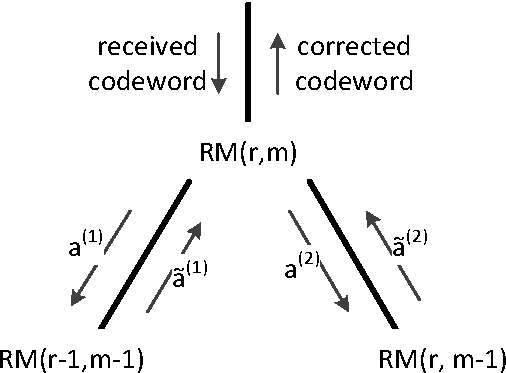
\includegraphics[width=4.0in,height=2.2in]{GMC_node.pdf}
	\vspace{0.5cm}
\end{frame}

\begin{frame}
\frametitle{Decoding Algorithm}
\framesubtitle{The Recursive Decoding Algorithm}
	\vspace{0.5cm}
	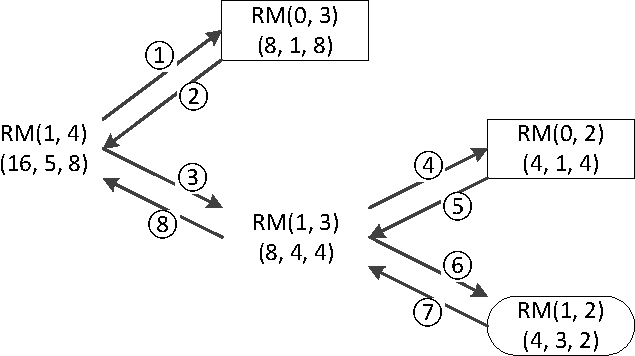
\includegraphics[width=4.2in,height=2.5in]{Baum_RM14_Ablauf.pdf}
	\vspace{0.5cm}
\end{frame}


\section{Conclusion}
\begin{outlineframe}
	\tableofcontents[currentsection]
\end{outlineframe}
\begin{frame}
Trapdoor\\
\vspace{0.3cm}
Encoding based on PUF-response\\
\vspace{0.3cm}
The hardness of LPN problem\\
\vspace{0.3cm}
Hash Function \\
\vspace{0.3cm}
Decoding with error correction algorithm\\
\end{frame}	


\section{Schedule}
\begin{outlineframe}
	\tableofcontents[currentsection]
\end{outlineframe}
\begin{frame}
	\vspace{0.3cm}
	\centering
	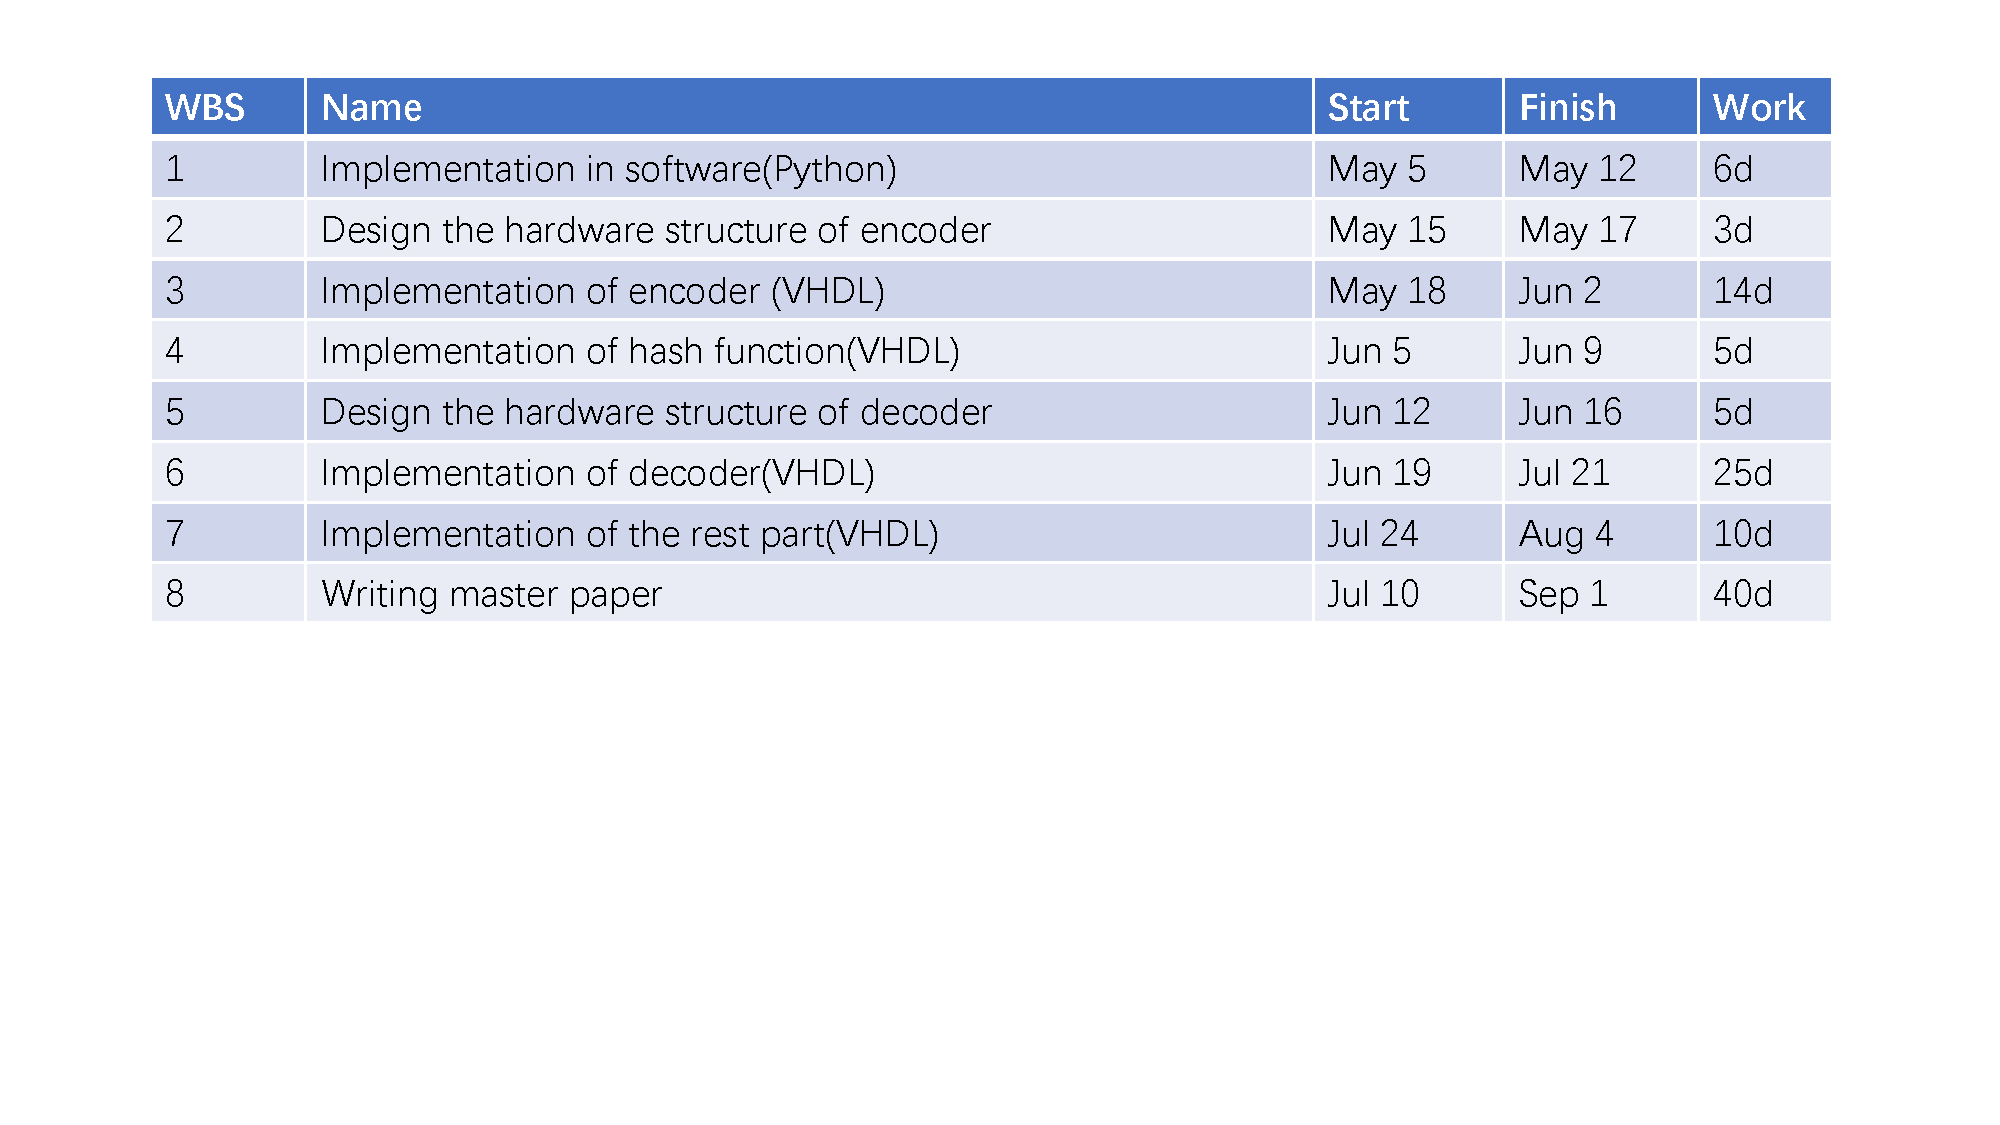
\includegraphics[width=5in,height=3.8in]{Schedule.pdf}
\end{frame}	



\section{Bibliography}
\begin{outlineframe}
	\tableofcontents[currentsection]
\end{outlineframe}
\begin{bibliographyframe}
$[1]$ A. Blum, A. Kalai, and H. Wasserman, “Noise-tolerant learning, the parity problem, and the statistical query model,” J. ACM, vol. 50, no. 4, pp. 506–519, 2003.\\
$[2]$ V. Lyubashevsky, “The parity problem in the presence of noise, decoding random linear codes, and the subset sum problem,” in Proc. 8th Int. Workshop Approximation, Randomization Combinatorial
Optimization Algorithms Techn., 2005, pp. 378–389.\\
$[3]$ E. Levieil, and P.-A. Fouque, “An improved LPN algorithm,” in Proc. 5th Int. Conf. Security Cryptography Networks, 2006, pp. 348–359.\\
$[4]$ Bossert, Martin: Kanalcodierung. 3., überarb. Aufl. München : Oldenbourg, 2013. – XVIII, 531 S. : graph. Darst.. – ISBN 978–3–486–72128–7 – 978–3–486–75516–9 
\end{bibliographyframe}

\section{Discussion}
\begin{outlineframe}
	\tableofcontents[currentsection]
\end{outlineframe}
\begin{frame}
	\frametitle{Discussion}
	\center{{\Large Question? }}\\	
\end{frame}	

\begin{frame}
	\frametitle{Post-quantum cryptography}
	Post-quantum cryptography refers to cryptographic algorithms (usually public-key algorithms) that are thought to be secure against an attack by a quantum computer.\\
	Post-quantum cryptography is distinct from quantum cryptography, which refers to using quantum phenomena to achieve secrecy and detect eavesdropping.\\
	
	
	
	
	
	
	When calculate the subcode of RM-Code, the information-bits s can also be calculated;\\
	
	the analysis of decoding complexity of RM-Code\\
	
	
	
	
\end{frame}	



\begin{contactframe}
    \contactpage
\end{contactframe}

\end{document}
